\documentclass[11pt, a4paper,titlepage]{article}
\usepackage[a4paper,top=1.5cm,bottom=1.5cm,left=2cm,right=2cm]{geometry}
%% Declaro simbolo
\usepackage[T1]{fontenc}
\newcommand{\rmfont}[1]{{\fontfamily{ptm}\selectfont%
#1}}
\newcommand{\rmfontbf}[1]{{\fontfamily{ptm}\selectfont%
\textbf{#1}}}
\newcommand{\rmfontsc}[1]{{\fontfamily{ptm}\selectfont%
\textsc{#1}}}

%%----------------------------------------------------

	\usepackage[spanish]{babel}
	\selectlanguage{spanish}
   
	\usepackage[utf8]{inputenc} % Aca va el setup para el codigo.
    \usepackage{graphicx}
    \usepackage{upquote}% esto tampoco creo
    \usepackage{amsmath,array,siunitx}
    \newcommand{\vvert}[1]{\left\Vert #1\right\Vert}
    \usepackage{listings}
	\usepackage{mdframed}
	\usepackage{xcolor} 
    \usepackage[utopia]{mathdesign}
    \newcommand{\Matlab}{\rmfont{\sc Matlab}}
    \newcommand{\Adina}{{\sc ADINA}}
    \newcommand{\refp}[1]{(\ref{#1})}
    \newcommand{\unspace}{\!\!\!\!\!\!\!\!\!\!\!\!\!\!\!\!\!\!\!\!}
    \newcommand{\ms}{\ \ \ } %Matrix Spacing
    \newcommand{\di}{\textrm{d}}
    \newcommand{\jac}{\rmfontbf{J}}
    \newcommand{\Djac}{|\;\jac\;|}
    \newcommand{\dNi}{\di N_i}
    \newcommand{\sigmab}{\boldsymbol{\sigma}}
    \newcommand{\varepsilonb}{\boldsymbol{\varepsilon}}
    \newcommand{\Phib}{\boldsymbol{\Phi}}
    \newcommand{\Omegab}{\boldsymbol{\Omega}}
    \newcommand{\COmega}{\boldsymbol{\{ } \Omega \boldsymbol{\} }}
    \newcommand{\CPhi}{\boldsymbol{\{ } \Phi \boldsymbol{\} }}
    \newcommand{\Mme}[1]{\boldsymbol{[}\mathbf{#1} \boldsymbol{]}}
    \newcommand{\Mmes}[1]{\boldsymbol{[}\boldsymbol{ \mathrm{#1} }\boldsymbol{]}}
    \newcommand{\Rme}[1]{\boldsymbol{\lfloor}\mathbf{#1} \boldsymbol{\rfloor}}
    \newcommand{\Cme}[1]{\boldsymbol{\{ }\mathbf{#1} \boldsymbol{\}} }
    \newcommand{\MB}{\Mme{B}}
    \newcommand{\MN}{\Mme{N}}
    \newcommand{\ME}{\Mme{E}}
    \newcommand{\Mk}{\Mme{k}}
    \newcommand{\MA}{\Mme{A}}
    \newcommand{\radial}{r}
    \newcommand{\eff}{f}
    \newcommand{\modal}{{_{\Phib}}}
    \newcommand{\dampfact}{\varsigma}
    
\newmdtheoremenv[% ACA PODES MODIFICAR LAS PROPIEDADES DEL CODIGO {code}
font=\fontsize{12pt}{16pt},
linecolor=black,
leftmargin=-.9cm,%
rightmargin=-.9cm,
backgroundcolor=gray!5,%
innertopmargin=8pt,%
ntheorem]{code}{Codigo}[section]
%-----------------------------------------------------------
% Code
%\newcommand{\feaPP}{codep1.tex}
%\newcommand{\feaSP}{codep2.tex}
%\newcommand{\feaTP}{codep3.tex}
%\newcommand{\annexFile}{annex.tex}
%\newcommand{\feaQP}{codep4.tex}
%No code
\newcommand{\feaPP}{null.tex}
\newcommand{\feaSP}{null.tex}
\newcommand{\feaTP}{null.tex}

\newcommand{\feaQP}{null.tex}
\newcommand{\annexFile}{null.tex}

\begin{document}  %Aqui empieza el documento
\begin{titlepage} %Esta es la caratula
\centering
{\scshape\Huge Elementos Finitos Cheatsheet \par}
\vspace{1cm}

\vspace{2cm}
{\scshape\Large\textbf{Autores} \par}
\medskip %medskip,smallskip,vspace son todos comandos para dejar espacio en blanco entre cosas
 \textsc{55423}

\end{titlepage} %Termina la caratula


\input{\feaPP}

\section{Parcial 2}
Protip: Necesitas saber que fuerza se tiene que hacer para que se mantenga en posición una arista o punto dado cargas térmicas/fuerza? Apoyalo (fix) y mira las reacciones con la carga termica/fuerza.
\subsection{Expresiones útiles}

\begin{align}
    \sigma_{v}&=\sqrt{\sigma_{x}^2+\sigma_{y}^2+\sigma_{z}^2 - \sigma_x \sigma_y-\sigma_x\sigma_z -\sigma_y \sigma_z +3(\sigma_{xy}^2+\sigma_{xz}^2 +\sigma_{yz}^2)} \\
    \sigma_{v}&=\sqrt{\tfrac{1}{2}\left[  (\sigma_{11}-\sigma_{22})^2+(\sigma_{11}-\sigma_{33})^2+(\sigma_{22}-\sigma_{33})^2\right] +3(\sigma_{12}^2+\sigma_{13}^2 +\sigma_{23}^2)}
\end{align}

\begin{equation}
    \lambda = \frac{E \nu}{(1+\nu)(1-2\nu)} \qquad\quad \mu=G=\frac{E}{2(1+\nu)}
\end{equation}

\begin{equation}
\begin{bmatrix}
    \sigma_{xx} \\
    \sigma_{yy} \\
    \sigma_{xy}
\end{bmatrix}
={\frac{E}{1-\nu^2}} 
\begin{bmatrix}
    1 & \nu & 0 \\
    \nu & 1 &0 \\
    0 & 0 & \frac{1-\nu}{2}
\end{bmatrix}
\cdot
\begin{bmatrix}
    \varepsilon_{xx} \\
    \varepsilon_{yy} \\
    2\varepsilon_{xy}
\end{bmatrix}
\end{equation}

\begin{equation}
\begin{bmatrix}
    \sigma_{11} \\
    \sigma_{22} \\
    \sigma_{12}
\end{bmatrix}
={\frac{E}{(1+\nu)(1-2\nu)}} 
\begin{bmatrix}
    1-\nu & \nu &0 \\
    \nu &1-\nu& 0 \\
    0 & 0 & \frac{1-2\nu}{2}
\end{bmatrix}
\cdot
\begin{bmatrix}
    \varepsilon_{11} \\
    \varepsilon_{22} \\
    2\varepsilon_{12}
\end{bmatrix}
\end{equation}

\begin{equation}
    \sigma_{n}=\frac{\sigma_{xx}+\sigma_{yy}}{2}+\left(\frac{\sigma_{xx}-\sigma_{yy}}{2}\right)\cos 2\theta +\tau_{xy}\sin 2\theta 
\end{equation}

\begin{equation}
    \tau_{n}=-\left(\frac{\sigma_{xx}-\sigma_{yy}}{2}\right)\sin 2\theta +\tau_{xy}\cos 2\theta 
\end{equation}

\begin{equation}
    I=\int^1_{-1} \phi(\xi) \di \xi \approx \phi(\xi_1) W_1+\phi(\xi_2) W_2 \ldots \phi(\xi_n) W_n
\end{equation}
\begin{equation}
    I=\int^1_{-1} \int^1_{-1}\phi(\xi,\eta) \di \xi \di \eta\approx \sum_i \sum_j W_i W_j\phi(\xi,\eta) 
\end{equation}



\begin{tabular}{>{$n=$}l<{ \vspace{10pt}}*{13}{c}}
0 &&&&&&&1&&&&&&\\
1 &&&&&&$x$&&$y$&&&&&\\
2 &&&&&$x^2$&&$xy$&&$y^2$&&&&\\
3 &&&&$x^3$&&$x^2y$&&$xy^2$&&$y^3$&&&\\
4 &&&$x^4$&&$x^3y$&&$x^2y^2$&&$xy^3$&&$y^4$&&\\
5 &&$x^5$&&$x^4y$&&$x^3y^2$&&$x^2y^3$&&$xy^4$&&$y^5$&\\
6 &$x^6$&&$x^5y$&&$x^4y^2$&&$x^3y^3$&&$x^2y^4$&&$xy^5$&&$y^6$
\end{tabular}

\begin{figure}
    \centering
    \includegraphics[width=0.5\textwidth]{fig/pascalsTetra.eps}
    \caption{El tetrahedro de Pascal. Los términos de los elementos \textit{serendipidad} están encuadrados.}
    \label{fig:PascalsTetrahedron}
\end{figure}

\subsection{Como obtener cualquier función de forma}
Se define cuantos nodos se va tener por elemento y se los ubica en el espacio $(\xi,\eta)$ que por simplicidad se trataran como $(x,y)$. Con el triangulo de Pascal para polinomios se elige el grado del polinomio y los términos. Luego se resuelve el sistema de ecuaciones $N_i\cdot X= A$ donde $N_i=[N_1\ms N_2 \ms \ldots\ms N_n]$ y $X=[1\ms x\ms y \ms\ldots\ms x^{k-1}y^{k} \ms x^{k}y^{k}]^T$, o algo por el estilo. Se tienen que elegir los grados mas convenientes teniendo en cuenta la simetría y el número de nodos, este ultimo te limita el número de términos posibles por la naturaleza de la interpolación. La matriz $A$ tendrá en su \textbf{espacio fila} el mismo polinomio evaluado en la posición del nodo correspondiente a esa fila.

\[
A=
\begin{bmatrix}
    1 & x_1 & y_1 & \dots  & x_{1}^{k-1}y_1^{k} & x_{1}^{k}y_1^{k} \\
    1 & x_2 & y_2 & \dots  & x_{2}^{k-1}y_2^{k} & x_{2}^{k}y_2^{k} \\
    \vdots & \vdots & \vdots & \ddots & \vdots& \vdots \\
    1 & x_n & y_n & \dots  & x_{n}^{k-1}y_n^{k} & x_{n}^{k}y_n^{k}
\end{bmatrix}
\]
Luego, las funciones de forma $N_i$ se pueden obtener así: $N_i=X^{-1} A$

\subsection{Elementos isoparamétricos}
\begin{itemize}
    \item Un elemento que no esta distorsionado (sigue siendo rectangular) tiene $J$ constante
    \item Cuidado con modo espurio. Ver tabla 6.8-1 pg. 226 el tema de full/reduced integration.
    \item Todo sobre como cargar tu elemento isoparam. en pg. 228
    \item 
\end{itemize}

\begin{figure}[htb!]
    \centering
    \includegraphics[width=12cm]{fig/gauss_n3.eps}
    \caption{Puntos gauss para ordenes $n=2$ y $n=3$. El peso para $n=2$ es igual en todos los puntos $W_i=1$}
    \label{fig:gauss_n3}
\end{figure}
\subsection{Ejemplo elemento exótico}
\subsubsection*{Matriz de Rigidez}
Imaginemos un elementos Q5 cuadrado de $2\times2$ con espesor $t$  (igual al Q4 con un nodo en su centro). Si fuéramos a obtener las funciones de formas de dicho elemento quedarían iguales para $(x,y)$ y para $(\xi,\eta)$ por las dimensiones usadas. La funcionalidad que uno estaría tentado a seleccionar sería $[1\ x \ y\ x^2 \ y^2 ]$, pero está trae problemas inesperados debido a que tiene varias soluciones en la interpolación. Como nuestra prioridad siempre es mantener la simetría la funcionalidad será $[1\ x\ y\ xy\ x^2y^2 ]$.  Tomando el orden de la figura \ref{fig:elemq5}.
\[
N_i=\left[\begin{array}{ccccc} \frac{x^2\,y^2}{4}+\frac{x\,y}{4}-\frac{x}{4}-\frac{y}{4}, & \frac{x^2\,y^2}{4}-\frac{x\,y}{4}+\frac{x}{4}-\frac{y}{4}, & \frac{x^2\,y^2}{4}+\frac{x\,y}{4}+\frac{x}{4}+\frac{y}{4}, & \frac{x^2\,y^2}{4}-\frac{x\,y}{4}-\frac{x}{4}+\frac{y}{4}, & 1-x^2\,y^2 \end{array}\right]
\]

Llegado a este punto nos interesa obtener la matriz de rigidez. Si queremos lograr \emph{``full integration"} deberíamos usar Gauss orden $n=3$ según $2n-1\geq O\left(\MB^T \ME \MB \right)$. El producto $\MB^T \ME \MB$ da un polinomio de orden 6 ($\MB$ tiene el mismo orden que la derivada de $\MN$). De esta forma nos aseguramos que nuestro resultado va ser exacto para el elemento sin distorsionar.

Para esté ejemplo, no se pide \emph{full integration} entonces no pasa nada si queremos \emph{underintegrate}. Usamos Gauss orden $n=2$. 

\begin{figure}[htb!]
    \centering
    \includegraphics[height=5cm]{fig/exoticElement.eps}
    \caption{Elemento Q5 rectangular.}
    \label{fig:elemq5}
\end{figure}

La rigidez de un elemento está dada por 


\begin{equation}
    \Mk=\int \MB^T \ME \MB \di V=\iint \MB^T \ME \MB t \di x \di y=\int^1_{-1}\int^1_{-1} \MB^T \ME \MB t \ \Djac \  \di\xi  \di\eta
\end{equation}
donde $\MB$ es la matriz deformación-desplazamiento del elemento, $\ME$ es la matriz constitutiva, y $\Djac$ es el determinante de la matriz Jacobiana, el cual se le suele decir simplemente el Jacobiano.

Este ultimo se calcula a partir de la derivada de las funciones de forma $ $

\subsubsection*{Cargas 2-D}
La ecuación que rige como se cargan elementos, siendo $\Cme{r}$ las cargas nodales, $\Cme{F}$ fuerzas volumétricas, $\CPhi$ fuerzas de tracción superficiales, $\Cme{\varepsilonb_0}$ las deformaciones iniciales y $\Cme{\sigmab_0}$ las tensiones iniciales (pg. 228)
\begin{equation} \label{eq:CargasGenerales}
    \Cme{r}=\int \MN^T \Cme{F} \di V +\int \MN^T \CPhi \di S+\int \MB^T \ME \Cme{\varepsilonb_0} \di V- \int \MB \Cme{\sigmab_0} \di V
\end{equation}
\textbf{Carga de linea}. Si el elemento está cargado sobre la linea 4-3 con una distribuida $q(x)$ (en [\si{\newton \per \meter}]) entonces procedemos de la siguiente manera según el segundo término de \refp{eq:CargasGenerales}: 

\begin{align}
    r_{xi}&=\int^1_{-1}N_i (\tau \jac_{11}- \sigma \jac_{12})t\di \xi \\
    r_{yi}&=\int^1_{-1}N_i (\sigma \jac_{11}+\tau \jac_{12})t \di \xi 
\end{align}
    donde $\sigma$ es la solicitación normal a la superficie y $\tau$ es la tangencial. Para la fuerza sobre el nodo 4 se tiene
    
    $$r_{y4}= N_4(\xi_2)t\left[\sigma(\xi_2)\; \jac_{11}+\tau(\xi_2)\; \jac_{12}\right] \cdot W_2 + N_4(\xi_3)t\left[\sigma(\xi_3)\; \jac_{11}+\tau(\xi_3)\; \jac_{12}\right]\cdot W_3 $$

    Si consideramos que solo hay una \emph{carga distribuida de linea} a tracción/compresión como indica la figura \ref{fig:elemq5}, se reduce la ecuación anterior
    
    $$ r_{y4} = N_4(\xi_2)\;\jac_{11}\;q(\xi_2) + N_4(\xi_3)\;\jac_{11}\;q(\xi_3) =N_4\;q \;\jac_{11}\Big|_{\xi_2} + N_4\;q\; \jac_{11}\Big|_{\xi_3} $$
    similarmente $r_{y3} = N_3\;q \;\jac_{11}\big|_{\xi_2} + N_3\;q\; \jac_{11}\big|_{\xi_3} $ donde la matriz Jacobiana también se evalúa para cada punto de Gauss!
    
    \textbf{Carga volumétrica}. 
\subsubsection*{Tensiones}
    \begin{itemize}
        \item Las tensiones en los nodos suele ser de mayor interés que sobre los puntos de gauss (mas comprometidas, permiten estimar error)
    \end{itemize}
    \clearpage
 \input{\feaSP}
\section{Parcial 3}

\subsection{Axisimetría}
Resuelvo problema 3-D en el plano. Los resultados son por cada unidad radian. Como sigo teniendo dos grados de libertad tengo las mismas funciones de forma. Cambia mi operador derivada.
\[
\begin{Bmatrix}
    \sigma_\radial \\
    \sigma_\theta \\
    \sigma_z \\
    \tau_{z\radial}
\end{Bmatrix}
= \frac{(1-\nu)E}{(1+\nu)(1-2\nu)}
\begin{bmatrix}
   1 & \eff & \eff & 0 \\
    & 1 & \eff & 0 \\
    & & 1 & 0 \\
    \textrm{sim.}\unspace& & & g 
\end{bmatrix}
\left(
\begin{Bmatrix}
\varepsilon_\radial \\
\varepsilon_\theta \\
\varepsilon_z \\
\gamma_{\radial z}
\end{Bmatrix}
-
\begin{Bmatrix}
\alpha T\\
\alpha T \\
\alpha T \\
0
\end{Bmatrix}
\right)
\]
donde 
\[
f=\frac{\nu}{1-\nu}\qquad \quad \textrm{y}\quad \qquad g=\frac{1-2\nu}{2(1-\nu)}
\]

Una carga puntual $P$ aplicada sobre un elemento axisimétrico no tiene el mismo significado físico que en elementos plane stress/strain. 
\[
P=2\pi rq
\]
donde $q$ es la carga distribuida en [N/m], $r$ es la distancia al eje de revolución y $2 \pi$ es el resultado de integrar la fuerza distribuida sobre $\theta$. 

\[
\Cme{r_e} = \int\int_{-\pi}^{\pi} \MN^T \begin{Bmatrix}
    \rho r \omega ^2 \\
    0
\end{Bmatrix} r \di \theta \di A
\]

\subsection{Subestructuras}
\[
\begin{bmatrix}
    K_{AA} & K_{AB} \\
    K_{BA} & K_{BB}
\end{bmatrix}
\begin{bmatrix}
    D_A \\
    D_B
\end{bmatrix}
= \begin{bmatrix}
    R_A \\
    R_B
\end{bmatrix}
\]

\[ 
D_B = K_{BB}^{-1} (R_B - K_{BA}D_A)
\]
\[
D_A =K_{AA}^{-1}(R_A-K_{AB}D_B)
\]

\subsection{Pitfalls}
\subsubsection*{\Matlab{}}
\begin{itemize}
    \item Antes de aplicar carga distribuida, verificar la orientación del elemento con sus nodos ($\xi,\eta$)
    \item
\end{itemize}
\subsection{Error}
Tipos de error:
\begin{itemize}
    \item Modelado
    \item Bugs
    \item Error de usuario
    \item Error de discretización
    \item Error de redondeo/truncado
    \item Error de manipulación 
    \item Error numérico (combinación de los dos anteriores)
\end{itemize}

Cálculo Tensiones en puntos superconvergencia (Gauss orden 1 para Q4, y Gauss orden 2 aproxima para Q8).

Extrapolo tensiones superconvergentes a los nodos ($\sigma^*$).

Energía de deformación.

Se suele requerir que $\eta\leq 0,05$
\[
\vvert{U}^2 = \sum^m_{i=1}\int_{v_e} \Cme{\varepsilonb}_i^T \ME \Cme{\varepsilonb}_i \di V
\]
\[
\vvert{e}^2=\sum_{i=1}^m \int_{v_e} \left( \Cme{\varepsilonb^*}_i - \Cme{\varepsilonb}_i\right)^T \ME \left( \Cme{\varepsilonb^*}_i - \Cme{\varepsilonb}_i\right) \di V
\]

\[
\vvert{e}^2=\sum_{i=1}^m \int_{v_e} \left( \Cme{\sigmab^*}_i - \Cme{\sigmab}_i\right)^T \ME ^{-1} \left( \Cme{\sigmab^*}_i - \Cme{\sigmab}_i\right) \di V
\]

\[
\eta = \sqrt{\frac{\vvert{e}^2}{\vvert{e}^2+\vvert{U}^2}}
\]




\input{\feaTP}
\subsubsection*{\Adina}
\begin{figure}[htb!]
    \centering
    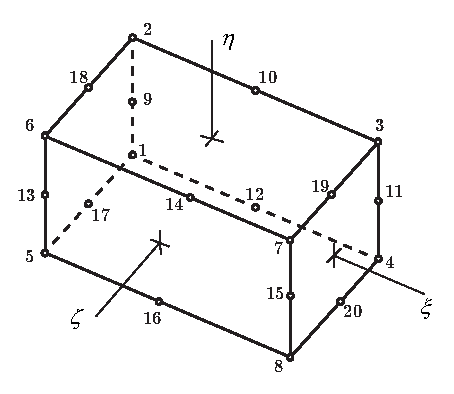
\includegraphics[width=.6\textwidth]{fig/H20numbering.eps}
    \caption{Numeración de nodos H20 en \Adina (Ejes sugeridos)}
    \label{fig:H20numbering}
\end{figure}

\section{Finitos II}
\begin{equation} \label{eq:vibraciones}
	\Mme{M}\Cme{\boldsymbol{\ddot{\mathrm{D}}}} + \Mme{C}\Cme{\boldsymbol{\dot{\mathrm{D}}}}+\Mme{K} \Cme{D} =\Cme{R}
\end{equation}
Amortiguamiento $\Mme{C} = \alpha \Mme{M}+\beta \Mme{K}$ cede una matriz no diagonal. Se complica la resolución. Existen dos otros modelos que tratan con una matriz $\Mme{C\modal}$ diagonal donde las ecuaciones se desacoplan.


Amortiguamiento Modal: Se elige un $\dampfact$ para cada modo
\begin{equation}
\Mme{C\modal}=\left[ \begin{array}{ccc}{2 \omega_{n} \dampfact_{n}} & {0} & {0} \\ {0} & {\ddots} & {0} \\ {0} & {0} & {2 \omega_{1} \dampfact_{1}}\end{array}\right]
\end{equation}

Amortiguamiento proporcional. Se basa el análisis 

\begin{equation}
	\Mme{C\modal} = \Mme{\Phib}^T ( \alpha \Mme{M}+\beta \Mme{K})\Mme{\Phib} = \alpha \delta \Mme{I} +\beta \Mme{\Omegab^2}
\end{equation}

Si se quiere estudiar un rango de frecuencias de excitación tal que $\omega_{\mathrm{exc}}\in [\omega_1, \omega_2]$ y eligiendo dos valores de damping para ambas frecuencias $\dampfact_1$ y $\dampfact_2$ se tiene:
\begin{align*}
\alpha &= 2\omega_1 \omega_2 (\dampfact_1 \omega_2 -\dampfact_2 \omega_1)/(\omega_2^2 - \omega_1^2) \\ \beta &= 2(\dampfact_2\omega_2 -\dampfact_1 \omega_1)/(\omega_2^2 - \omega_1^2)
\end{align*}

Una vez obtenida $\Mme{C\modal}$ se pueden obtener los desplazamientos modales $\Cme{Z}$. Tome en cuenta que debido a la diagonalidad de $\Mme{\Omegab^2}$ y $\Cme{R\modal }$ se desacoplan las ecuaciones de \ref{eq:vibraciones} y por ende se pasa a tratar dichas matrices diagonales como vectores columnas. Una vez desacopladas se tiene
 \[\Cme{\boldsymbol{\ddot{\mathrm{Z}}}}+2\COmega \Cme{C\modal} \Cme{\boldsymbol{\dot{\mathrm{Z}}}} + \COmega^2 \Cme{Z} = \Cme{R\modal} \]
\[
\Cme{Z} = \frac{\Cme{R\modal }}{{\COmega}^2 \sqrt{(1-\chi^2)^2 + (2 \Cme{C\modal} \chi)^2}}
\]
donde $\chi = \frac{\omega_{\mathrm{exc}}}{\COmega}$. 



\subsection{Sine Sweep}
A medida que la frecuencia de excitación aumenta la \textit{amplitud del sistema disminuye}\footnote{Excepto en cercanías de una frecuencia natural}. Es interesante pensar que si aumentara no tendría sentido buscar las frecuencias naturales porque estas son caracterizadas por un máximo de amplitud. Las curvas del barrido de frecuencia son decrecientes en lejanía de una frecuencia natural porque para una fuerza cíclica $F(t)=F_0\sin \omega t$ el tiempo que actúa en una dirección es inversamente proporcional a la frecuencia. Por ende la estructura no tiene tiempo para moverse lejos antes de que se invierta la dirección de la fuerza.



\section{Apuntes Segundo Parcial}

Es cuasiestatico cuando la deformacion avanza 

Cargas armonicas: Analizo respuesta de la estructura ante cada modo. 

Aumentar damping disminuye la amplitud del motor, pero a la vez lo que le otorga damping se convierte rigido y toma reacciones.

Para simular transitorio podemos usar la descomposicion modal con metodos numericos usando runge kutta... porque ahora tengo una particular... la funcion 

Ahora pueden variar de cualquier manera:
\[
D=D(x,y,z,t) = N(x,y,z)D(t)
\]

Desarrollamos $D$ en serie Taylor.

$f(x_0+\Delta x)= f(x_0) + f'(x_0) \Delta x +\tfrac{1}{2}...$

Con las ecuaciones de taylor despejadas para $n+1$ y $n-1$ puedo adivinar el futuro con el presente (y pasado).
\[
\{D\}{n+1}=\{D\}{n-1}+2 \Delta t\{\dot{D}\}_{n}
\]

Sin conocer $\dot{D}_{n}$ esta dificil... uso taylor otra vez!

\[
\left[\frac{M}{\Delta t^{2}}+\frac{C}{2 \Delta t}\right]\{D\}{n+1}=\left\{R^{e x t}\right\}{n}-[K]\{D\}{n}+\frac{2}{\Delta t^{2}}[M] \} D{n}-\left[\frac{M}{\Delta t^{2}}-\frac{C}{2 \Delta t}\right]\{D\}_{n-1}
\]

donde $\left\{ R^{e x t}\right\}$ puede ser una función en el tiempo también! Una funcion heaviside excita TODOS los modos.

Optimización: No hay mucho que se pueda hacer. Es super complicated

RUNGE KUTTA

Tengo que resolver las dos ecuaciones simultáneamente
\[
\left\{\begin{array}{l}{[M] \dot{V} \}+[C] V \}+[K]\{D\}=\left\{R^{\text {ert}}\right\}} \\ {\{\dot{D}\}=\{V\}}\end{array}\right.
\]

Espectro de respuesta


Gráfico $\ddot{u}$--$\omega$ muestra las cargas que podría estar sometido tu sistema.

A frecuencias mas altas la diferencia entre las Z es mayor:

\[
S_{i}=\frac{Z_{i}^{\text { mâx }}}{Z_{i}^{\text { st }}}
\]

Ataco el sistema con un ``Paquete`` de cargas y cada modo responde de su propia forma. Este metodo Sebas le dice Random. Se suele usar para sistemas tipo placas en satelites, donde tenes todas las plaquetas vibrando y no conoces que esta pasando ahi. Para estructuras no tanto porque son más estables y se conoce mejor que puede llegar a ser el modo de vibración porque los modos de vibracion estan bien separados-> cosa que no es verdad en satelites. 

\[
\mathrm{D}(\mathrm{t}){\mathrm{j}}=[\Phi]\{\mathrm{Z}(\mathrm{t})\}=\sum{\mathrm{j}} \Phi_{\mathrm{ji}} Z_{\mathrm{i}}(\mathrm{t})=\sum_{\mathrm{j}} \Delta_{\mathrm{ji}}(\mathrm{t})
\]



Voy a tener un desplazamiento máximo cuando los modos esten todos en su máximo... pero eso sucede cuando están en fase, cosa que nunca sucede porque siempre hay algun desfasaje. Hay criterios para determinar el desplazamiento máximo, una incluye sumando la primer autoforma que es la más grande y luego sumando cuadrados mínimos de las otras. Con esto te cubris de la tensión que podría llegar a ocurrir ().



\input{\feaQP}
\input{\annexFile}
\end{document} 




% \begin{comment}
%     \section{Dudas}
%     \begin{enumerate}
%         \item Pg. 223 Cook: $\Mk$ de un solido 8 nodos se integra con $n=2$, pero $\MB$ se integra con $n=3$. Pero se necesita $\MB$ para obtener $\Mk$.
%         \item Si quiero verificar calidad de un elemento, me basta con pararme arriba cada punto Gauss y verificar que $\Djac$ no sea igual a cero y que no cambie de signo?
%         \item Tengo un problema plain strain pero tengo $q(x)$ en [N/m]. No lo integro con $t$! No? Inversamente, para el mismo problema, si tengo solo presiones o fzas volumetricas puedo olvidarme que existe $t$ y no usarla para el calculo de la matriz rigidez (y presiones/fzas vol). Se le dice singularidad a un punto donde $\Djac$ es cero?
%         \item Si quiero tensiones en puntos Gauss, cambia la dimension de $\MB$ cuando itero sobre los puntos? Cook dice que $\MB$ is calculated from (lower order) displacement field. wtf?
%         \item \textbf{Follow-up} Cuando itero sobre los mismos Puntos de Gauss para obtener tensiones, cambian mis $\MN$? Sé que puedo usar los puntos de Gauss para extrapolar tensiones en los nodos, pero hablo antes de eso
%         \item Para un elemento me conviene siempre ser perfectamente simétrico en la elección del orden del polinomio? Hay alguna vez que voy a tomar $[1\ms x\ms y\ms xy\ms x^2]$ antes de tomar algo por el estilo de  $[1\ms x\ms y\ms y^2\ms x^2]$
%     \end{enumerate}
%     \end{comment}